\documentclass[14pt,Diplom]{diplomwork}

\usepackage{fancyvrb}
\renewcommand{\theFancyVerbLine}{\footnotesize\arabic{FancyVerbLine}}
\usepackage[dvips]{color}
\usepackage{tikz}
\usepackage{graphicx}
\graphicspath{{./img/}}

\newcommand{\alert}[1]{{\color{red}#1}}

\sloppy

\date{2022}
\author{студент МКб-4301-51-00}{Мельков Алексей Константинович}
\advisor{канд. физ.-матем. наук, доцент}{Марков Роман Владимирович}
\title{Разработка модуля интеграции онлайн-сервиса построения графиков и геометрических чертежей в визуальный онлайн HTML-редактор}


\napravlenie{02.03.01}{Математика и компьютерные науки}
\profile{Математические основы компьютерных наук}
\kafedra{фундаментальной математики}{Е.\,М.~Вечтомов}
\department{компьютерных и физико-математических наук}{Н.\,А.~Бушмелева}
\institute{математики и информационных систем}

% ЗАПОЛНЕНИЕ РЕФЕРАТА ПО НОВОМУ ОБРАЗЦУ
%TODO Обязательно впишите ключевые слова
\keywords{<ключевые слова>}

\annotation{
	\begin{description}
		\item[Объект разработки:] модуль интеграции онлайн-сервиса построения графиков и геометрических чертежей в визуальный онлайн HTML-редактор
		%TODO

		\item[Цель:] <Переносится цель ВКР дословно>
		%TODO

		\item[Методы проведения работы:] <Описываются применяемые методы: анализ научной литературы, сравнительный анализ, математическое моделирование, методы математического анализа и т.\,д.>
		%TODO

		\item[Рассматриваются вопросы:] связи онлайн-сервиса построения графиков и геометрических чертежей GeoGebra и визуальный онлайн HTML-редактор TinyMCE
		%TODO
	\end{description}





}
\regtotcounter{figure}
\regtotcounter{table}
\begin{document}

	
\maketitle
\makereferat		% печатаем реферат
\newpage

\tableofcontents


\Chapter{Введение}
Выпускная квалификационная работа посвящена разработке модуля интеграции онлайн-сервиса построения графиков и геометрических чертежей в визуальный онлайн HTML-редактор


\textbf{Актуальность} работы обусловлена оптимизацией времени и удобности написания статей, вопросов, заданий. Данный модуль позволит интегрировать распространенный онлайн-сервис построения графиков и геометрических чертежей GeoGebra в онлайн HTML-редактор TinyMCE, который также присутствует на платформе Moodle. Что добавит возможность составления новых тестов, лекций, практических заданий для обучения студентов.

\textbf{Объектом исследования} является изучение связи программ TinyMCE, GeoGebra, платформы Moodle. Для этого потребовалось рассмотреть их API и построение плагина	

\textbf{Предмет исследования}~--- 

\textbf{Цель работы:} написание плагина для платформ Moodle, который расширит возможности TinyMCE добавлением новой кнопки, которая сможет открыть сервис построения графиков GeoGebra.

Для достижения поставленной цели сформулированы следующие \mbox{\textbf{задачи:}}

\begin{enumerate}
	\item Изучение основ программирования на языке JavaScript
	\item Изучение API GeoGebra, TinyMCE
	\item Узнать как создается плагин для расширения TinyMCE на плафторме Moodle
	\item Создание плагина
\end{enumerate}



\textbf{Теоретическая значимость работы} состоит в следующем...

\textbf{Практическая значимость работы} состоит в следующем...

В целом работа носит \textbf{теоретический (или прикладной, или практический)} характер.



\textbf{Структура работы.} Выпускная квалификационная работа, общим объемом \pageref{LastPage}~стр., состоит из введения, двух глав, заключения, библиографического списка.

Первая глава посвящена теоритической части

Вторая глава посвящена практической части


В заключении представлены основные результаты дипломной работы.

В библиографический список включено (кол-во) источников.


Результаты работы \textbf{апробированы} (в докладах..., статьях ..., внедрены...)


\chapter{Теоретическая часть}

\section{JavaScript}

\paragraph{JavaScript}

это язык программирования. Поддерживает объектно-ориентированныйи стили.

JavaScript обычно используется как встраиваемый язык для программного доступа к объектам приложений. Наиболее широкое применение находит в браузерах как язык сценариев для придания интерактивности веб-страницам.

В своем модуле с помощью JavaScipt я связываю онлайн редактор с сервисом GeoGebra. Также с его помощью написан плагин, который добавляет кнопку в TinyMCE и вставляет график в его текстовую область. 

\paragraph{Синтаксис}
 это набор правил, по которым строится программа на JavaScript:
 \begin{itemize}
 	\item каждую строку надо заканчивать символом ';'
 	\item чтобы объявить переменную надо написать ее идентификатор (имя) и слово var или let
 	\item чтобы присвоить значение переменной надо испольхвоать знак '='
 	\item помимо переменных, существуют условия и циклы
 	\item для создания более сложных объектов есть методы (особые функции), они бывают встроенные самим языком, а также те, которые написали лично
\end{itemize}

\paragraph{}
Для того, чтобы интегрировать JavaScript код в HTML страницу надо вставить парный тег <script>. Но также можно подключить JS файл с помощью ссылки на него тем же тегом, использованием атрибута src, то есть надо указать где лежит этот файл.

\section{Cоздание плагина для TinyMCE на платформе Moodle}
Для создания плагина TinyMCE нужно сгенерировать каталог.

В нем минимум должны находитьcя:

\begin{itemize}
	\item Подкатолог /lang
	\item Подкатолог /pix
	\item Подкатолог /tinymce
	\item Файл lib.php
	\item Файл version.php
\end{itemize}

\paragraph{/lang}
 предназначен для хранения языковых папок. В моем примере в ней существует подкаталог /en в котором находится файл tinymce\_ИмяПлагина.php\\
 Файл обязан содержать запись\\
  \textcolor{orange}{<?php} \\
  \textcolor{blue}{\$string}[\textcolor{red}{'pluginname'}] = \textcolor{red}{'ИмяПлагина'};\\
  где 'pluginname' нельзя изменять.

\paragraph{/pix}
содержит иконку вашего плагина в расширении .png, обычно это 20 $\times$ 20 пикселей.

\paragraph{/tinymce}
оснвоной католог, содержащий js файл. В нем находится скрипт, что будет делать наш плагин.

\paragraph{lib.php}
содержит код плагина Moodle, здесь должен находиться по крайней мере класс tinymce\_ИмяПлагина с методом update\_init\_params()\\
 \textcolor{orange}{<?php} \\
 \textcolor{green}{defined}(\textcolor{red}{'MOODLE\_INTERNAL'}) || (\textcolor{green}{die});\\
 
\textcolor{green}{class} \textcolor{blue}{tinymce\_ИмяПлагина} \textcolor{green}{extends} editor\_tinymce\_plugin \{ \\
\textcolor{green}{protected} \textcolor{blue}{\$buttons} = \textcolor{green}{array} (\textcolor{red}{'ИмяПлагина'}); \\

\textcolor{green}{protected function} \textcolor{blue}{update\_init\_params}(\textcolor{green}{array} \& \textcolor{blue}{\$params}, context \textcolor{blue}{\$context}, \textcolor{green}{array} \textcolor{blue}{\$options} = \textcolor{green}{null}) \{ \\

\textcolor{blue}{\$this} -> \textcolor{yellow}{add\_button\_after}(\textcolor{blue}{\$params},3,\textcolor{red}{'ИмяПлагина'},\textcolor{red}{'spellchecker'});\\

\textcolor{blue}{\$this} ->\textcolor{yellow}{add\_js\_plugin}(\textcolor{blue}{\$params});\\

 \}\\
\}\\


 \paragraph{version.php}
 содержит информацию о версии плагина Moodle\\
  \textcolor{orange}{<?php} \\
 \textcolor{green}{defined}(\textcolor{red}{'MOODLE\_INTERNAL'}) || (\textcolor{green}{die});\\
 \textcolor{cyan}{\#текущая версия плагина (Дата: ГГГГММДДЧЧ)}\\
 \textcolor{blue}{\$plugin} -> \textcolor{brown}{version} = 2012112900; \\
 \textcolor{cyan}{\#требующиеся версия Moodle (Дата: ГГГГММДДЧЧ)}\\
 \textcolor{blue}{\$plugin} -> \textcolor{brown}{requires} = 2012112900; \\
 \textcolor{cyan}{\#полное имя плагина}\\
 \textcolor{blue}{\$plugin} -> \textcolor{brown}{component} = \textcolor{red}{'tinymce\_ИмяПлагина'}; \\
 
В итоге мы должны получить примерно такой каталог:\\

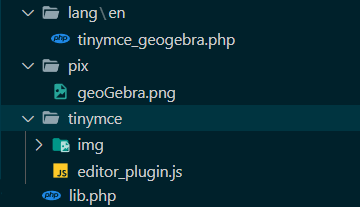
\includegraphics[width=0.5\linewidth]{1.png}



 
\chapter{Однако, глава}
\section{и раз}
\subsection{и два}
\subsubsection{и три}
\begin{figure}[H]
	\caption{sdfgsdfgsf}
	\label{fig:wqewe}
\end{figure}

\begin{table}[H]
	\caption{sdfgsdfgsf}
	\label{tbl:wqewe}
	\begin{tabular}{|c|c|}
		\hline
		a & b \\
		\hline
		a & b \\
		\hline
		a & b \\
		\hline
	\end{tabular}
\end{table}


\Chapter{Заключение}



\begin{thebibliography}{99}
\bibitem{Book1} \alert{Библиография оформляется по ГОСТ 7.0.5-2008} 
\bibitem{Book2} \alert{Библиография оформляется по ГОСТ 7.0.5-2008} 
\end{thebibliography}

\APPENDIX
\chapter{Листинг программы}
\linespread{1}

%1.Функция,  котороя перемножает коэффициенты многочлена на матрицу:
\begin{Verbatim}[numbers=left,firstnumber=last,fontsize=\small]
f(x, F) := block([i, S], 
    S: zeromatrix(dim, dim), 
    for i: 1 thru length(F) do
        S: S+mod(F[i]*(x^^(i-1)), P), 
    return(mod(S, P))
);
\end{Verbatim}  


\end{document}
